\chapter{MARCO DE REFERENCIA}\label{ch:marco_de_referencia}

En este capítulo se detallan los antecedentes del proyecto, la descripción 
del problema abordado, los objetivos generales y específicos, las limitaciones, y se hace una 
revisión del estado del arte referente a la simulación de procesos de estampado utilizando 
el método de los elementos finitos.

\section{Antecedentes}

Los procesos de estampado forman  parte importante de la industria metal-mecánica, muchas 
piezas metálicas se fabrican utilizando estos procesos, debido a los altos volúmenes de 
producción y a la rapidez de fabricación respecto a otros métodos como la fundición, forja 
o el mecanizado. Es empleado en gran variedad de sectores: electrodomésticos ,
automotriz, aeronáutico, naval, electrónico e informático y su objetivo es aprovechar al máximo 
el material para elaborar la mayor cantidad de piezas con el menor tiempo y costo posible. \\

El proceso de estampado, es vital dentro del sector automotriz en México, genera una demanda 
de mercado con un valor de unos \$17,000 millones de dólares. Este monto es conformado por la 
suma de la proveeduría nacional, que aporta \$6,000 millones de dólares y las importaciones de 
piezas y componentes que utilizan este proceso de manufactura, valuadas en poco más de 
\$11,000 millones de dólares. Esto significa que la proveeduría nacional (fabricantes en el país) 
abastece el 35.2\% de la demanda que se presenta dentro de dicho proceso de la cadena de valor 
del sector automotriz. ~\cite{elhorizonte} \\

Las operaciones de troquelado y estampado pueden parecer actividades en las cuales no hay mayor 
ciencia o desarrollo de ingeniería, y muchas veces, los herramentales utilizados 
se fabrican mediante una aproximación dada por la experiencia de un jefe de taller o un 
mecánico matricero, y posteriormente se realizan pruebas para ajustar en donde sea necesario.
Está claro que para una industria pequeña esto puede funcionar, dado que la exigencia 
en la producción y las pérdidas económicas derivadas de un diseño inadecuado son mínimas. 
Pero, normalmente, en las industrias del sector automotriz los requerimientos en tiempo y 
costo dejan menos margen de maniobra e implican que los procesos de diseño sean desarrollados 
mediante una metodología que garantice la disponibilidad del producto en tiempo y forma.\\

En ese contexto, las herramientas computacionales, es decir paquetes de software CAD, CAE o CAM, 
proporcionan una ventaja competitiva considerable, puesto que permiten a las empresas agilizar 
los procesos de diseño y manufactura de los herramentales utilizados, que 
en conjunto con los procedimientos de producción y los aspectos de logística, posibilitan  
establecer una metodología ágil para el desarrollo de nuevos productos o de los ya existentes.


% Actualmente para garantizar el desarrollo a tiempo de un producto es necesario 

% La posibilidad de desarrollar simulaciones de los procesos de estampados metálicos fue 
% durante mucho tiempo casi una utopía para la industria. Los ingenieros 
% de procesos esperaban ser capaces de identificar posibles defectos en el formado en etapas 
% tempranas de diseño y/o desarrollo de los herramentales, y minimizar la necesidad de 
% modificaciones costosas de las herramientas en una serie de procesos de ensayo y error.\\


\section{Planteamiento del problema}

La empresa Bypasa S.A. de C.V. diseña y fabrica componentes utilizados en partes antivibratorias, 
para el sector automotriz, específicamente bujes y abrazaderas utilizadas en las suspensiones, 
partiendo desde la formulación de los materiales poliméricos requeridos, la selección de la geometría 
y la validación del diseño. Sin embargo los herramentales: moldes y troqueles, que utiliza en sus 
procesos de producción son diseñados y fabricados por empresas extranjeras y/o nacionales. Por esto 
se desarrolló un proyecto cuyo objetivo fue poner en operación un centro de diseño, fabricación 
y validación de moldes y troqueles.\\

El modelado y simulación, por medio de métodos numéricos computacionales, de los procesos de fabricación 
involucrados en el desarrollo de los herramentales es una parte importante del proyecto, puesto que 
permitirá tomar decisiones respecto a los diseños en etapas tempranas, minimizando los costos derivados de 
los ajustes realizados después de ejecutar \textit{corridas} de prueba.\\

Por lo tanto el problema que tiene la empresa es que no cuenta con la implementación de herramientas 
CAD/CAE para el diseño de herramentales y por ello se requiere realizar la simulación del proceso de formado de un 
tubo de acero que será fabricado con un troquel diseñado en el nuevo centro de desarrollo, 
con la finalidad de determinar la forma de la geometría final del producto, comparar con las especificaciones, 
precisar si es necesario un rediseño, además de obtener algunos datos de interés como la fuerza de formado 
requerida para completar el proceso.

\section{Justificación}

El desarrollo de este proyecto permitirá establecer una metodología de trabajo, que incluya herramientas computacionales 
de simulación por elementos finitos, para el diseño, manufactura y validación de troqueles formadores. Impactando directamente 
en los recursos de la empresa, debido a la reducción en los costos y tiempos de fabricación de herramentales, inherentes a cuando 
se tienen proveedores externos. Posibilitando, consecuentemente, que el desarrollo de nuevos productos para partes estampadas 
se puedan realizar en periodos más cortos, lo cual brinda una ventaja competitiva.

% La simulación por elemento finito en el proceso de diseño de herramentales, así como en 
% la simulación de procesos de estampado es una herramienta muy útil, puesto que representa un ahorro 
% significativo de costos y tiempo, a la vez que permite establecer una metodología de trabajo más efectiva, minimizando las 
% actividades de tipo prueba-error para la realización de ajustes.\\

% Además de lo anterior, la simulación presenta la ventaja de poder variar parámetros que influyen en los procesos de 
% estampado, de manera conveniente, sin que esto derive en gastos excesivos de recursos, con la finalidad de entender 
% de mejor manera la influencia de ciertas propiedades o condiciones, e inclusive optimizar las características 
% de un componente.

\section{Objetivo general}

Simular el proceso de formado de un tubo de acero AISI 1018 utilizando el método de los elementos finitos 
y validar los resultados obtenidos mediante la técnica de extensometría.

\section{Objetivos particulares}
\begin{itemize}
\item Simular utilizando el método de los elementos finitos el proceso de formado del tubo.
% \item Identificar fallas potenciales o características no deseables en el tubo.
\item Comparar resultados obtenidos de simulaciones utilizando una condición de deformación plana y un análisis tridimensional.
\item Validar los resultados de la simulación mediante la técnica de extensometría.
% \item Verificar las características geométricas y dimensionales del tubo.
%%% \item Caracterizar de forma experimental y por elemento finito el comportamiento elástico de la materia prima utilizada.
\end{itemize}


\section{Alcances}

Los alcances de este proyecto comprenden el desarrollo de un modelo de elemento finito del proceso de 
formado, con la posterior realización de la simulación mediante un enfoque dinámico-explícito. Además, 
de la validación experimental de la simulación utilizando la técnica de extensometría.

% \begin{itemize}
% \item Desarrollo de un modelo de elemento finito del proceso de formado del tubo.
% \item Simulación del modelo utilizando un análisis tipo dinámico-explícito.
% \item Validación de la simulación.
% % \item Publicación de un artículo.
% \end{itemize}


\section{Estado del arte}

La posibilidad de desarrollar simulaciones de los procesos de estampados metálicos fue durante mucho tiempo 
un deseo inalcanzable para la industria de estampados. Los ingenieros de procesos esperaban ser capaces de 
identificar posibles defectos en el formado en etapas tempranas de diseño y/o desarrollo de los herramentales, 
y minimizar la necesidad de modificaciones costosas de las herramientas en una serie de procesos de ensayo y error. \\

El modelado de problemas de estampado de partes metálicas requiere una precisión considerable en la caracterización 
de efectos como el comportamiento no lineal de un material, grandes deformaciones y condiciones de contacto entre la
herramienta y la parte a estampar que derivan  en algoritmos complejos.\cite{banabic2000}\\

La primera formulación teóricamente correcta de problemas de formado de metales fue presentada por 
Wang y Budiansky ~\cite{wang1978} en 1978. El método presentado fue una formulación total lagrangiana 
e involucraba elementos triangulares membrana de deformación constante. La solución implementada fue 
un esquema incremental Euleriano hacia adelante. Los métodos basados en un 
esquema de solución como el anterior son llamados como métodos estáticos-explícitos. \\

En el inicio de la década de los 90's hubo un incremento considerable en la utilización de la simulación de estampado 
metálico dentro de la industria y a mediados de esta década la mayoría de las compañías en la industria automotriz 
establecieron las simulaciones de estampado como aspectos elementales en el desarrollo de sus procesos.
Los códigos de tipo dinámico explícito dominaron el mercado, programas de propósito general como LS-DYNA y 
Abaqus/Explicit, además de programas especializados como PAM-STAMP y OPTRIS \cite{banabic2000}.
Actualmente existen programas de computadora altamente especializados en la simulación de estampados entre los 
cuales se ecuentran AutoForm y STAMPACK, adémás de los de propósito general como ANSYS, LS-DYNA, Abaqus, 
NASTRAN, entre otros.\\

La simulación de procesos de estampado es una práctica extentendida sobre todo en los países industrializados y 
aplicado de manera dominante en procesos de embutición profunda, el cual es un proceso de deformación un poco 
más complejo que las operaciones de doblado tratadas en este trabajo de tesis. Enseguida se describen de 
manera somera algunos trabajos realizados sobre simulación de estampados.\\

Jorge Olivera en ~\cite{olivera2014} describe una metodología analítica y la simulación numérica de un doblado en U 
utilizando un software comercial de elementos finitos. De la simulación numérica obtuvo las variaciones de espesor 
y el estado de esfuerzos (figura \ref{fig:olivera}) de la pieza conformada.

\begin{center}
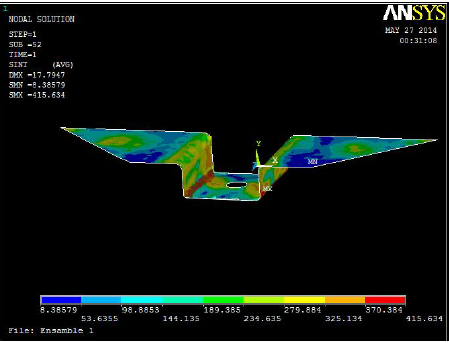
\includegraphics[width=0.7\textwidth]{src/ch1/olivera.png}
\captionof{figure}{Estado de esfuerzos para el análisis realizado por Olivera \cite{olivera2014}}
\label{fig:olivera}
\end{center}

Natalia García en \cite{garcia2009} realizó una simulación por elementos finitos del proceso de 
embutición de una chapa que sirve como pieza de soporte de la llanta de repuesto de un automóvil. 
Utilizó un enfoque dinámico explícito para la simulación. El análisis realizado consta 
de 4 etapas, realizadas progresivamente, para cada una de las cuales ejecutó varios análisis 
variando las propiedades del material utilizado, así como las velocidades de trabajo, con la 
finalidad de obtener una velocidad de embutición adecuada y la reducción del peso de la pieza.\\

Arwidson \cite{arwidson2005} realizó una comparación del comportamiento de cuatro materiales (aceros de
alta resistencia) en un proceso de estampado mediante una simulación por elementos finitos
utilizando dos software: PamStamp y LS-DYNA. Lo anterior buscando encontrar un modelo 
numérico y las condiciones de frontera adecuadas para el proceso, además de simular
el fenómeno de la recuperación elástica (springback) utilizando Abaqus, para determinar la
sobre-deformación a aplicar con el herramental. De acuerdo a los resultados, Arwidson estima
que las mayores deformaciones se sobrevaloran en alrededor de un 75 \% en las regiones sometidas 
a flexión crítica. Reporta también que la variación del coeficiente de fricción en el rango 
de 0 a 0.1 tiene una influencia casi nula en la simulación del proceso de estampado. \\

% \begin{center}
% 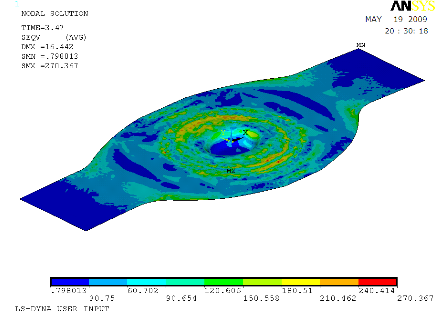
\includegraphics[width=0.6\textwidth]{src/ch1/garcia2009.png}
% \captionof{figure}{Estado de esfuerzos esquivalentes en pieza analizada por García \cite{garcia2009}}
% \label{fig:garcia2009}
% \end{center}

Lindberg \cite{lindberg2012} evaluó la implementación de un software de simulación por elemento finito 
(LS-DYNA) en el proceso de diseño de herramentales de la compañía Duroc Tooling, buscando
reducir los grandes costos derivados de errores en el proceso de diseño. Desarrolló un modelo
de elemento finito para un elemento estructural producido mediante un proceso de estampado, 
y evaluó los beneficios reportados por la simulación: tales como la identificación de grietas,
arrugas o cualquier tipo de debilitamiento en la chapa. Respecto a la parte económica hace
hincapié en el costo de una licencia de un software de este tipo, resultando redituable para 
cuando una compañía desarrolla más de una decena de herramentales anualmente, si por el
contrario desarrolla unas pocas herramientas, entonces resultaría mejor pagar a una empresa
externa por cada simulación.\\

Para la simulación numérica de procesos de formado de tubo mediante doblados sucesivos en UO, 
similares al proceso a desarrollar, se tienen algunos trabajos anteriores, en la mayoría de los 
casos son autores japoneses que desarrollaron códigos con un enfoque elasto-plástico.\\

Makinouchi \cite{makinouchi1989} desarrolló un código de computadora para analizar un proceso 
de deformación por doblado en UO bajo condiciones de deformación plana, obteniendo resultados 
satisfactorios y sobre todo un algoritmo muy eficiente.\\

Huang & Leu ~\cite{huang1995} desarrollaron un código de análisis elasto-plástico por elemento finito, 
basado en una formulación lagrangiana modificada, para simular proceso de doblado UO en placas metálicas, 
bajo condiciones de deformación plana. Para realizar el análisis del proceso completo, dividieron este 
en tres pasos de carga o configuraciones que se muestran en la figura ~\ref{fig:pasos_formado_01}, 
doblado en U, descarga y doblado final en O. Aplicaron además simetría debido a la disposicion de las 
herramientas y el blank a formar, simplificando aún más el análisis. Utilizaron un coeficiente 
de fricción de $\mu = 0.02$ y el espesor de la chapa fue de 6 mm. \\
% En la figura ~\ref{fig:shape_sequence} 
% se puede observar la secuencia del desarrollo de la geometría obtenida mediante el análisis realizado. \\

\begin{center}
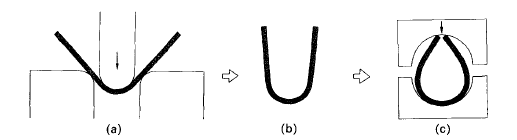
\includegraphics[width=0.75\textwidth]{src/ch1/uo-bending.png}
\captionof{figure}{Proceso de doblado UO, a) Doblado en U b) Descarga c) Doblado en O \cite{huang1995}}
 \label{fig:pasos_formado_01}
\end{center}

% \begin{center} \label{fig:shape_sequence}
% 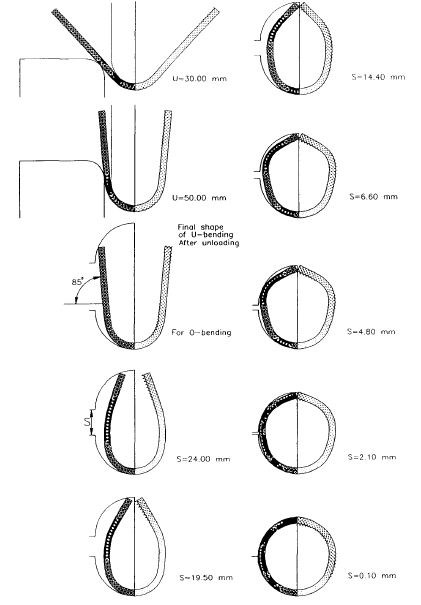
\includegraphics[scale=0.75]{src/ch1/shape_sequence.png}
% \captionof{figure}{Secuencia obtenida mediante el proceso de doblado UO. \cite{huang1995}}
% \end{center}

Chen y Huang ~\cite{chen2007} de manera similar a ~\cite{huang1995} simularon un proceso de doblado 
UO, con las mismas etapas: doblado en U, descarga y doblado en O. El espesor de lámina de la pieza 
de trabajo fue de 6 mm y un ancho de 10 mm. Utilizaron una ecuación exponencial para la relación 
esfuerzo-deformación. Los resultados obtenidos fueron la distribución 
de esfuerzos de von Mises y la forma geométrica resultante, medidas para ciertos intervalos 
de desplazamiento del punzon formador superior. \\

% \begin{center}
% 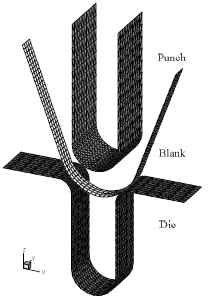
\includegraphics[scale=0.65]{src/ch1/u_bend.png}
% \captionof{figure}{Modelo de elementos finitos del doblado en U \cite{chen2007}}
% \label{fig:u_bend}
% \end{center}

% \begin{center}
% 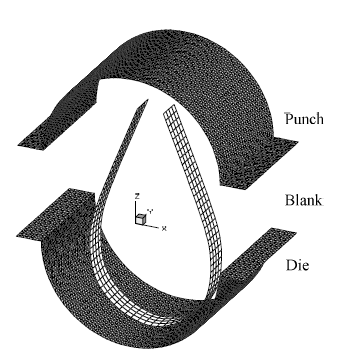
\includegraphics[scale=0.65]{src/ch1/o_bend.png}
% \captionof{figure}{Modelo de elementos finitos del doblado en O \cite{chen2007}}
% \label{fig:o_bend}
% \end{center}

Finalmente , García \cite{garcia2005} desarrolló un modelo de predicción del ángulo de recuperación y del 
radio de doblado final en procesos de doblado al aire, combinando técnicas de procesamiento digital 
de imágenes para el procesamiento y obtención de datos de la parte experimental, y el uso de redes neuronales 
para calcular el modelo de predicción a partir de la introducción de datos experimentales. En un enfoque 
similar, Rodríguez \cite{rodriguez2014} trabajó en el desarrollo de un modelo matemático que utilizó para 
optimizar parámetros de un doblado en U mediante las técnicas de nubes de partículas y algoritmo  genético, 
con la finalidad de obtener una relación que describiera de mejor manera el comportamiento de la recuperación 
elástica.